\section{鼓膜振动}
我们将鼓膜的振动近似地看作是一个有限大的圆形薄膜的二维振动,且不考虑周期力。
首先考虑一个矩形薄膜,其尺寸为$L_x$和$L_y$,边缘固定,表面张力系数T始终恒定。假设薄膜材料的面密度为$\sigma$。
\begin{figure}[h]
	\centering %图片居中
	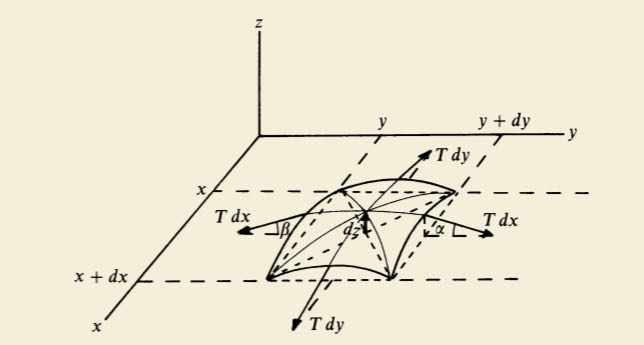
\includegraphics[width=0.6\textwidth]{pic/pic1} %设置大小为0.6倍文字宽度,大括号内为图片路径
	\caption{鼓上微元受力} %标题
	\label{fig.1}	%引用的编号
\end{figure}
薄膜发生振动时,考虑一面元dxdy,如图\ref{fig.1}所示,在竖直方向上有dz大小的位移,因此微元四周受到表面张力T给面元恢复平衡的趋势。其中垂直x轴方向的张力大小为$T\text{d}x$,它们的垂直分量为$-T\sin\alpha\text{d}x$和$-T\sin\beta\text{d}x$。$\alpha$和$\beta$为表面张力与水平面的夹角,小量近似得:
$$\sin\alpha\approx\tan\alpha=(\frac{\partial z}{\partial y})_{y+\text{d}y}$$
$$\sin\beta\approx\tan\beta=(\frac{\partial z}{\partial y})_y$$

因此这组张力的垂直分量有
$$F_y=-T\text{d}x\left[\left(\frac{\partial z}{\partial y}\right)_{y+d y}-\left(\frac{\partial z}{\partial y}\right)_y\right]=-T\text{d}x\frac{\partial^2 z}{\partial y^2}\text{d}y$$

同理,作用在面元上的垂直y轴方向的一组张力的垂直分量有
$$F_x=-T\text{d}y\frac{\partial^2 z}{\partial x^2}\text{d}x$$

则面元受到的竖直方向表面张力大小有$F=F_x+F_y$,根据牛顿第二定律有
$$T \text{d} x \text{d} y\left(\frac{\partial^2 z}{\partial x^2}+\frac{\partial^2 z}{\partial y^2}\right)=\sigma \text{d} x \text{d} y \frac{\partial^2 z}{\partial t^2}$$

两边除以$\text{d}x\text{d}y$得偏微分方程
$$\frac{\partial^2 z}{\partial t^2}=c^2\left(\frac{\partial^2 z}{\partial^2 x}+\frac{\partial^2 z}{\partial y^2}\right)$$

其中$c=\sqrt{\frac{T}{\sigma}}$,作极坐标代换得
$$\frac{\partial^2 z}{\partial t^2}=c^2\left(\frac{\partial^2 z}{\partial r^2}+\frac{1}{r} \frac{\partial z}{\partial r}+\frac{1}{r^2} \frac{\partial^2 z}{\partial \theta^2}\right)$$

\subsection{法一}

对z进行分离变量得$z=f(r)g(\theta)h(t)$,将上式代入二阶偏微分方程得
$$f(r) g(\theta) h^{\prime \prime}(t)=c^2\left(f^{\prime \prime}(r) g(\theta) h(t)+\frac{1}{r} f^{\prime}(r) g(\theta) h(t)+\frac{1}{r^2} f(r) g^{\prime \prime}(\theta) h(t)\right)$$

两边同时除以$f(r)g(\theta)h(t)$得
$$\frac{h^{\prime \prime}(t)}{h(t)}=c^2\left(\frac{f^{\prime \prime}(r)}{f(r)}+\frac{1}{r} \frac{f^{\prime}(r)}{f(r)}+\frac{1}{r^2} \frac{g^{\prime \prime}(\theta)}{g(\theta)}\right)$$

由于方程中右式仅与$t$相关,左式仅与$r\text{、}\theta$相关,且$t\text{、}r\text{、}\theta$是三个独立变量,则等式两边须等于同一个常数$-\omega^2$,于是得到两个方程$$h^{\prime \prime}(t)=-\omega^2 h(t)$$
$$\frac{f^{\prime \prime}(r)}{f(r)}+\frac{1}{r} \frac{f^{\prime}(r)}{f(r)}+\frac{1}{r^2} \frac{g^{\prime \prime}(\theta)}{g(\theta)}=-\frac{\omega^2}{c^2}$$

解得
$$h(t)=H \sin (\omega t+\Phi)$$

其中$H\text{、}\Phi$为常数,将化简后偏微分方程两边同乘$r^2$得
$$r^2 \frac{f^{\prime \prime}(r)}{f(r)}+r \frac{f^{\prime}(r)}{f(r)}+\frac{\omega^2}{c^2} r^2=-\frac{g^{\prime \prime}(\theta)}{g(\theta)}$$

由于方程中右式仅与$r$相关,左式仅与$\theta$相关,且$r\text{、}\theta$是两个独立变量,则等式两边仍须等于同一个常数,则可能为正弦函数或指数函数,而的周期为$2\pi$,则常数的公因数为一整数n的平方,则有
$$g^{\prime \prime}(\theta)=-n^2g(\theta)$$

解得
$$g(\theta)=G \sin (n \theta+\psi)$$

其中$G\text{、}\psi$为常数,于是偏微分方程有$$r^2 \frac{f^{\prime \prime}(r)}{f(r)}+r \frac{f^{\prime}(r)}{f(r)}+\frac{\omega^2}{c^2} r^2=n^2$$

两边同乘$f(r)$并除以$r^2$得
$$f^{\prime \prime}(r)+\frac{1}{r} f^{\prime}(r)+\left(\frac{\omega^2}{c^2}-\frac{n^2}{r^2}\right) f(r)=0$$

该方程的解为$J_n(\frac{\omega r}c)$和$Y_n(\frac{\omega r}c)$的线性组合,当r趋于0时,后者趋于-∞,于是膜中心为一奇点,则解仅与$J_n(\frac{\omega r}c)$有关\footnote{参见 吴崇试,高春媛.数学物理方法[M].北京大学出版社,2019.}。

由z的变量分离得
$$z=A J_n\left(\frac{\omega r}{c}\right) \sin (\omega t+\Phi) \sin (n \theta+\psi)$$

其中A为常数。则圆形薄膜的固有振动的频率有
$$f_{n, k}=\frac{j_{n, k}}{2 \pi a}c$$

其中$j_{n,k}$为n阶Bessel函数的第k个零点,a为鼓膜半径,$c=\sqrt{\frac{T}{\sigma}}$。

鼓的基频有
$$f_{0, 1}=\frac{j_{0, 1}}{2 \pi a}c$$

\subsection{法二}
偏微分方程和边界条件有
\begin{equation}
	\frac{\partial^2 z}{\partial t^2}=c^2 \left(\frac{\partial^2 z}{\partial r^2}+\frac{1}{r}\frac{\partial z}{\partial r}+\frac{1}{r^2} \frac{\partial^2 z}{\partial\theta^2}\right)
	\label{1.1}
	\tag{1.1}
\end{equation}

\begin{equation}
	\left .\mathrm{z}\right |_{r=0}\text{有界,}\left .\mathrm{z}\right |_{r=a}=0
	\label{1.2}
	\tag{1.2}
\end{equation}
\begin{equation}
	\left .z\right |_{\theta=0}=\left .z\right |_{\theta=2 \pi},\left .\frac{\partial z}{\partial \theta}\right |_{\theta=0}=\frac{\partial z}{\partial \theta} |_{\theta=2 \pi}
	\label{1.3}
	\tag{1.3}
\end{equation}

若方程有非零解
\begin{equation}
	z(r, \theta, t)=v(r, \theta) e^{i \omega t}
	\label{2}
	\tag{2}
\end{equation}

代入偏微分方程(\ref{1.1})及边界条件(\ref{1.2})和(\ref{1.3}),并令得下列偏微分方程本征值问题
\[
\begin{array}{c}
	\frac{1}{r} \frac{\partial}{\partial r}\left(r \frac{\partial v}{\partial r}\right)+\frac{1}{r^2} \frac{\partial^2 v}{\partial \theta^2}+k^2 v=0\\
	\left .v\right |_{r=0}\text{有界,}\left .v\right |_{r=a}=0\\
	\left .v\right |_{\theta=0}=\left .v\right |_{\theta=2 \pi},\left .\frac{\partial v}{\partial \theta}\right |_{\theta=0}=\left .\frac{\partial v}{\partial \theta}\right |_{\theta=2 \pi}
\end{array}
\]

再令$v(r,\theta)=R(r)\Theta(\theta)$,分离变量,分解为两个常微分方程的本征值问题
\begin{equation}
	\theta^{\prime \prime}(\theta)+\lambda \theta(\theta)=0 
	\label{3.1}
	\tag{3.1}
\end{equation}
\begin{equation}
	\theta(0)=\theta(2 \pi), \theta^{\prime}(0)=\theta^{\prime}(2 \pi)
	\label{3.2}
	\tag{3.2}
\end{equation}
和
\begin{equation}
	\frac{1}{r} \frac{d}{d r}\left[r \frac{d R(r)}{d r}\right]+\left(k-\frac{\lambda}{r^2}\right) R(r)=0
	\label{4.1}
	\tag{4.1}
\end{equation}
\begin{equation}
	\mathrm{R}(0)\text{有界,}R(a)=0
	\label{4.2}
	\tag{4.2}
\end{equation}

其中本征值问题(3)的解为
\[
\begin{array}{c}
\text{本征值}\lambda_m=m^2, m=0,1,2,3,\ldots\\
\text{本征函数}\Theta_m(\theta)=\left\{\begin{array}{l}\cos m \theta, \quad m=0,1,2, \ldots \\ \sin m \theta, \quad m=1,2,3, \ldots\end{array}\right.
\end{array}
\]
故本征值问题(4)中参数$\lambda=m^2$已知,本征值$k^2$待求
将(\ref{4.1})式两端乘以$rR^*(r)$再积分得$$k^2 \int_0^a R(r) R^*(r) r d r=m^2 \int_0^a R(r) R^*(r) \frac{d r}{r}+\int_0^a \frac{d R(r)}{d r} \frac{d R^*(r)}{d r} r d r$$
故一定有本征值$k^2>0$,通过作变换$x=kr$将微分方程(\ref{4.1})化为Bessel方程,从而求得它的通解$$R(r)=C J_m(k r)+D N_m(k r)$$
考虑到边界条件(\ref{4.2})的要求,$R(0)$有界,故$D$有界。又由于要求$R(a)=0$,得到$$J_m(ka)=0$$
将m阶Bessel函数的第i个正零点(由大到小排列)记作$\mu^{(m)}_i,i=1,2,3,\ldots$,则本征值问题(4)的解是
\[
\begin{array}{c}
\text{本征值}k_{mi}^2=(\frac{\mu^{(m)}_i}a)^2, i=1,2,3,\ldots\\
\text{本征函数}R_{mi}(r)=J_m(k_{mi}r)
\end{array}
\]
于是求得圆形薄膜的固有振动的频率,其中$\mu^{(m)}_i$是m阶Bessel函数的第i个正零点。

\section{定音鼓的发声机理简要分析}

\subsection{综述}
在定音鼓(timpani, or Kettledrum)的研究中,有几个重要的点需要强调。一是鼓上膜的振动模态,二是鼓腔内空气和膜共同振动,三是演奏时敲击的位置(影响哪种模态可以被激发)\upcite{fletcher2012physics}。
虽然空腔的形状和物理性质似乎也会改变频率,但研究表明这似乎不是一个非常重要的影响因素。
\subsection{鼓膜的影响}
由第一部分的理论计算我们可以知道,膜为圆形的鼓上,其模态为Bessel函数(普通、球形)的线性叠加(当然,膜为矩形或方形的鼓面也是存在的,葡萄牙的女性就常常演奏一种名叫\textit{adufe}的传统方形手鼓,但是我们暂时只研究圆形鼓面情况)。代入边界条件,通过求这些方程的数值解,可以得级数n不同时的振动模态\footnote{数值解仍旧参见吴书。}。
%Bessel函数数值解
\begin{table}[h]
    \centering
	\label{tab.1}
	\caption{前几级Bessel函数的数值根}
    \begin{tabular}{l|lllll}
    \toprule
        k & $J_0$ & $J_1$ & $J_2$ & $J_3$ & $J_4$\\ \midrule
        1 & 2.40483 & 3.83171 & 5.13562 & 6.38016 & 7.58834\\ \hline
        2 & 5.52008 & 7.01559 & 8.41724 & 9.76102 & 11.06471\\ \hline
        3 & 8.65373 & 10.17347 & 11.61984 & 13.01520 & 14.37254\\ \bottomrule
    \end{tabular}
\end{table}
%鼓膜振动模态
\begin{figure}[h]
	\centering %图片居中
	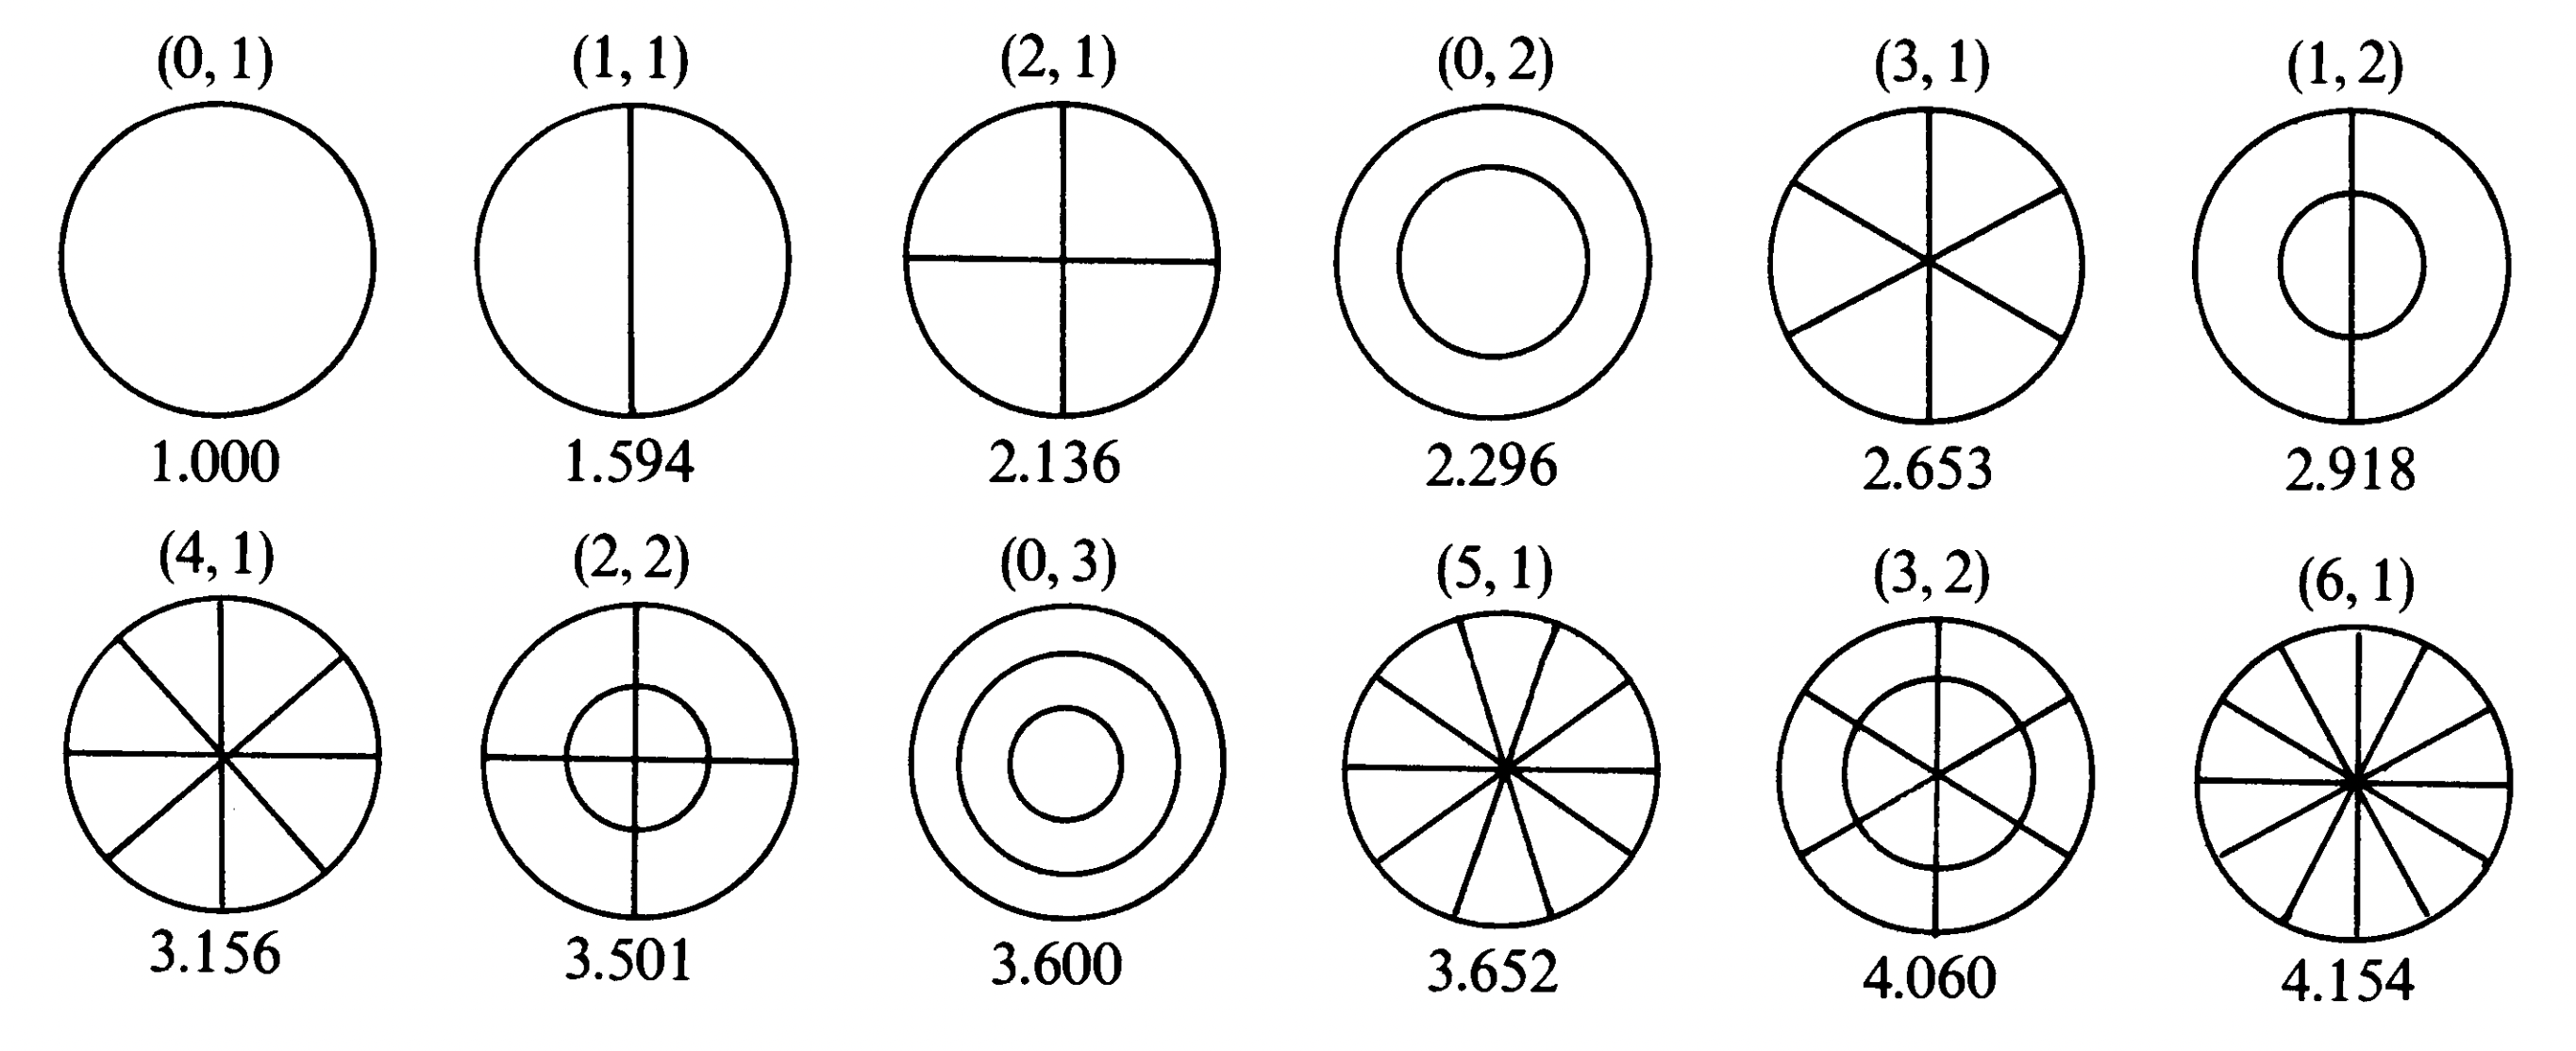
\includegraphics[width=\textwidth]{pic/pic2} %设置大小为0.6倍文字宽度,大括号内为图片路径
	\caption{前14个膜振动模态\upcite{fletcher2012physics}。以$f_{0,1}=\frac{j_{0,1}}{2\pi a}\sqrt{\frac{T}{\sigma}}=\frac{2.40483}{2\pi a}\sqrt{\frac{T}{\sigma}}$为基频,其他模态$(n,k)=\frac{f_{n,k}}{f_{0,1}}$} %标题
	\label{fig.2}	%引用的编号
\end{figure}

以(1,1)=1.594作基频,由上表作一些计算,(1,1):(2,1):(3,1)=1.00:1.34:1.66。但是实际测量发现经过调节后的定音鼓中的(1,1)、(2,1)和(3,1)模式的频率几乎为1:1.5:2\upcite{rossing1976acoustics}。(4,1)和(5,1)模式的比例通常为基本(1,1)模式的2.44倍和2.90倍(在2.5和3的半音范围内)。因此,1至5级的模态频率比接近2:3:4:5:6,这就是定音鼓有一种“音高感”的部分原因,即鼓面的振动频率本身就近似是简单整数比。

\subsection{空气的影响}
上面我们把(1,1)作为基频,实际上这是图\ref{fig.2}中画出的第二个模态。那为什么(0,1)模态不是基频?实际上,在一个封闭的鼓腔内,(0,1)的振动依赖于空气的压缩、膨胀而不是鼓面的振动(从图中它是唯一没有图案的可以直观地看出这一点)。我们知道,空气自带质量,其惯性会降低振动频率,这种效应在振动模态的级数比较低时尤为明显。所以人耳难以觉察这个频率,反而是比它高一级的(1,1)频率成为了事实上的基频\upcite{benson2006music}。虽然也有理论认为,Timpani鼓的底部小孔才是使(0,1)模式急剧衰减的重要因素,但这个理论已经被实验所否定。

还有关于(1,1)、(2,1)和(3,1)三者频率比的问题,之所以理论上膜的频率比和实际鼓的频率的测量值有较大差距,空气起了重要调音作用。我们可以粗略地说:

(1)腔内空气的弹性恢复力提高了同心模式 [(0,1)、(0,2)、(0,3) 等] 的频率;

(2)腔内空气的质量降低了其它模式 [(1,1)、(2,1)、(3,1) 等]的频率;

理论推导见下。

先估算一下量级,考虑频度$f=300$ Hz,尺度$a=0.25$ m,$v=300$ m/s,故空气对应波长较长,采取近场近似。
对(0,k):
$$\frac{\partial^2 z}{\partial t^2}=c^2\left(\frac{\partial^2 z}{\partial x^2}+\frac{\partial^2 z}{\partial y^2}\right)+\frac{\delta p}{\sigma}$$
$$\delta p=-\gamma \frac{p_0}{V_0} \delta V=-\gamma \frac{p_0}{V_0} S x_{0 k} A_{0 k}$$
其中
$$x_{0 k}=\frac{\int J_0(x) x\text{d}x}{\int x\text{d}x}=\frac{2}{\mu_{0 k}} J_1\left(\mu_{0 k}\right)$$
代入
$$z=A_{0 k} J_0\left(\omega_{0 k} t / c\right) \sin (\omega t)$$
得到
$$\omega^2=\omega_{0 k}^2+\gamma \frac{p_0 S}{\sigma V_0} x_{0 k}$$
$$\frac{\omega^2}{\omega_{0 k}^2}-1=\frac{\gamma p_0  \pi a^4 x_{0 k}}{T V_{0 k}} \sim \frac{p_0 a^4}{T V_0} \sim \frac{p_0 a}{T}$$

对(1,1),将空气视作低速流体:
$$\frac{\Delta E_k}{E_k}=\frac{1 / 2\left(\int \rho_a \omega z x \text{d}x\text{d}y\right)^2 / \rho V_0}{1 / 2 \int \sigma \omega^2 z^2\text{d}x\text{d}y}=\frac{\rho_a a^4}{\sigma V_0} \frac{\left(\int J_1(x) x^2 \text{d}x\right)^2}{\int J_1^2(x)x\text{d}x}$$
$$1-\frac{\omega^2}{\omega_{o k}^2} \sim \frac{\rho_a a^4}{\sigma V_0} \sim \frac{\rho_a a}{\sigma}$$

容易发现,对的不同n频率,同样有附加质量效应,随着n的增大,空气位移逐渐减小,附加质量逐渐减小。在较低的几个频率,空气的附加质量较大,于是通过控制定音鼓参数,可以调节其频率比率(1,1):(2,1):(3,1)=1.00:1.34:1.66。调节附加质量后比值(1,1):(2,1):(3,1)=1:1.5:2,此时构成协和音程。关于不同模态的表格参见图\ref{fig.4}。

除此之外,空气的一个重要作用是防止鼓上表面的振动通过它传递到下表面,后者形状和发声性质都未知,会引入其他的杂音。故空气层保证绝大多数能量都用于上表面振动发声,使鼓声从上表面向四周辐射开去,同时确保频率的“单一性、纯粹性”\upcite{loy2011musimathics}。
%打击点影响
\begin{figure}[h]
	\centering %图片居中
	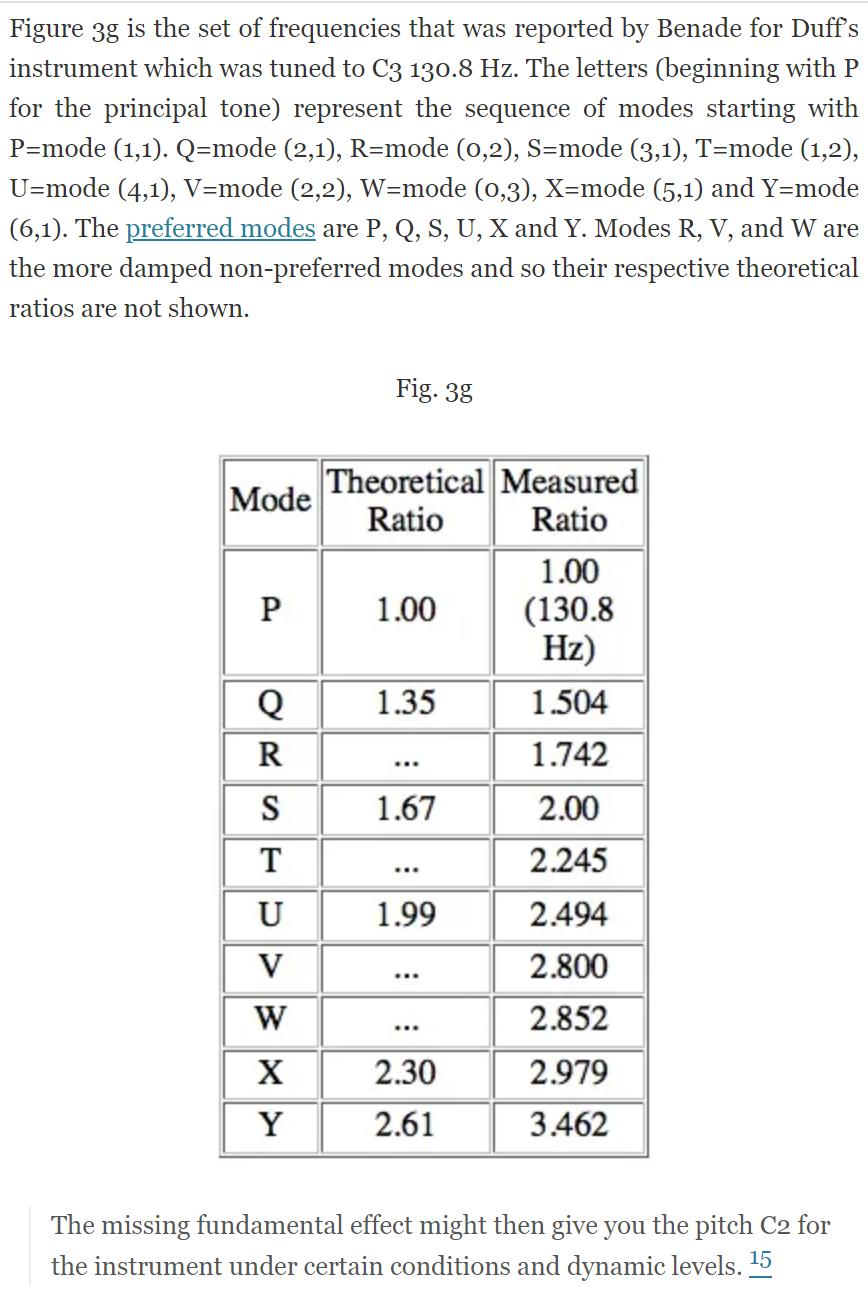
\includegraphics[width=0.45\textwidth]{pic/pic5} %设置大小为0.45倍文字宽度,大括号内为图片路径
	\caption{不同模态\upcite{benade1976fundamentals}}
	\label{fig.4}	%引用的编号
\end{figure}
\subsection{打击点的影响}
敲击边缘和中心对频率的激发存在一定的影响。例如敲击标准打击位置(从边缘起,到中央连线上的第一个四分点),可以保证(1,1)、(2,1)和(3,1)模态非常突出,而(0,0)仅仅和高级次的(4,1)差不多一样不显著,(0,2)更是比(5,1)稍弱(见图\ref{fig.3}(a)(b))。
打击中央点,虽然(0,1)、(0,2)较上次明显许多(图\ref{fig.3}(c)(d)),但两者衰减得也快。经过多次实验,研究者发现(1,1)、(2,1)等衰减最慢,故在Timpani的特例下,频率的激发几乎总是那么几个音高,故可以达到“定音”的效果。
%打击点影响
\begin{figure}[t]
	\centering %图片居中
	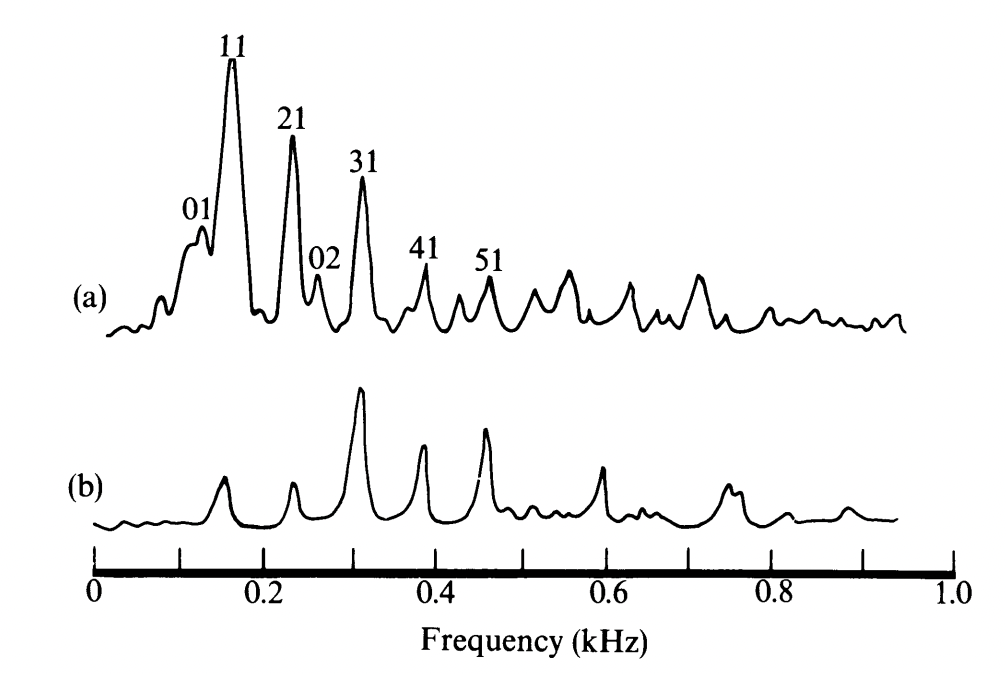
\includegraphics[width=0.45\textwidth]{pic/pic3} %设置大小为0.45倍文字宽度,大括号内为图片路径
	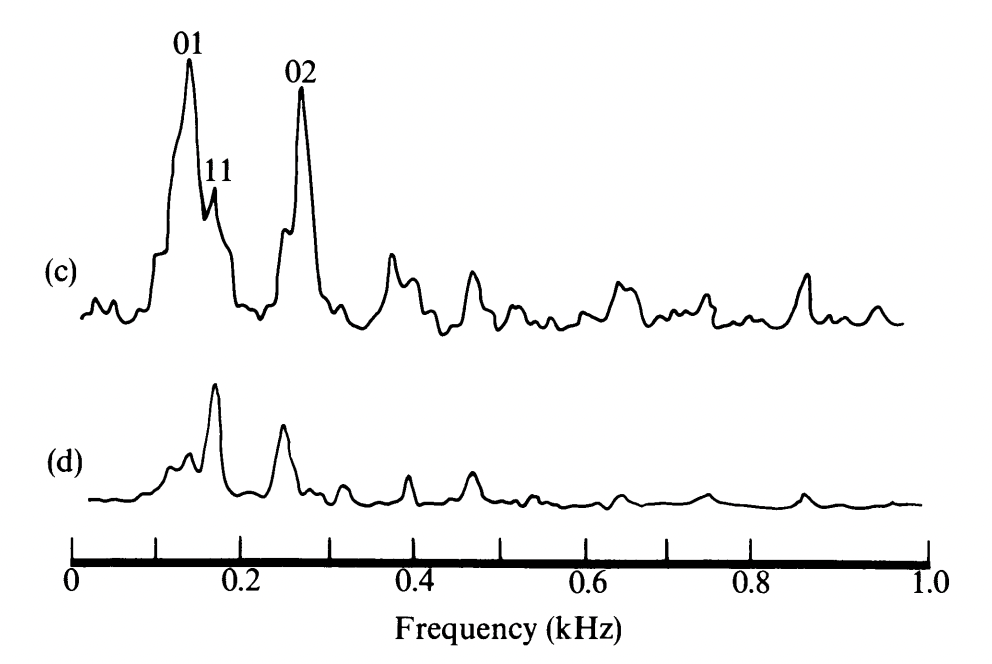
\includegraphics[width=0.45\textwidth]{pic/pic4}
	\caption{打击点影响,(a):敲击标准点后0.03 s;(b):敲击标准点后1 s;(c):敲击中央点后0.03 s;(d):敲击中央点后1 s。} %标题
	\label{fig.3}	%引用的编号
\end{figure}
\subsection{其他可能的影响因素}
空腔/鼓体的形状可以微调频率的高低,而包裹空腔的材质主要改变了音色。例如,形状相似的铜制的Timpani和合成材料制作的Timpani听起来差别巨大。膜的材料不同在声音性质层面可能也有些微的不同,例如小牛皮的音色更加悦耳,这可能与(0,1)频在小牛皮和其他材料上衰减速度不同有关。

\section{固定音高乐器和无固定音高乐器的本质区别}
在以上的讨论中,我们总是试图依据乐器的物理性质(材质、形状、边界条件等)来解出固定的振动模态。
其实,不管是什么类型的乐器,它们都有自己一定的振动模态。
但是,\textbf{固定音高乐器}一个重要的是特点是其模态在敲击(或者摩擦振动,这是弦乐器的情况)后保持一定,且除了泛音列和和声列之外不太会存在其他的杂波。
而\textbf{无固定音高乐器}(如很多噪音乐器)一方面设计时并没有像固定音高乐器一样严格确定尺寸、边界形状等等,另一方面实际演奏时就存在各种振动频率的随机叠加,而且某些情形下,波的频率还会随时间而改变。波形非常复杂,故人听不出一个固定的音高。

所以,两者本质区别在于能否发出频率固定的简单振动波形,并且允许与之频率比成近于简单整数比的其他固定频率波存在。
